\section{VMM Kernel Heap}
\subsection{Introducción}
Asi como existe la MMU que se encarga de administrar la memoria fsica, es decir, administrar los frames fsicos de 4kb, la unidad de memoria virtual esta encargada de administrar la memoria asignada 
de forma tal de poder otorgar punteros a sectores del tamao pedido. Bsicamente, nuestra vmm es una implementacin de malloc para uso del heap. No contamos con malloc para las tareas.

\subsection{Administracin del kernel heap}
La nica tarea que tiene soporte para uso de memoria dinnima en nuestro kernel es el mismo kernel. Para el manejo del heap se utiliza un mapeo especial dedicado al heap. La direccin donde se mapea 
el heap esta definida por KERNEL\_HEAP\_START (0xC0000000). Las funciones de la vmm se definen en vmm.h y vmm.c. La implementacin de kmalloc esta basada en la implementacin sugerida en 
\textit{The C language programming}, en la que el heap se administra en bloques de tamao variable. Cada bloque posee en su direccin ms baja la siguiente estructura:

\begin{verbatim}
union header{
    struct {
        //puntero al proximo bloque libre
        union header *ptr;
        //Tamao del bloque
        uint32_t size;       
    } s;
    
    //Solamente para alinear bien el header (el tipo align_t segun K&R puede variar segun la maquina)
    align_t x;
};
\end{verbatim}
Cada bloque de memoria del heap comienza con esta estructura, que es usada por kmalloc y kfree para saber donde est el prximo bloque de memoria 
libre, y que tamao tiene el bloque actual. De esta forma, la memoria fsica del heap queda estructurada como la siguiente figura:

\begin{figure}[H]
\centering
\subfloat{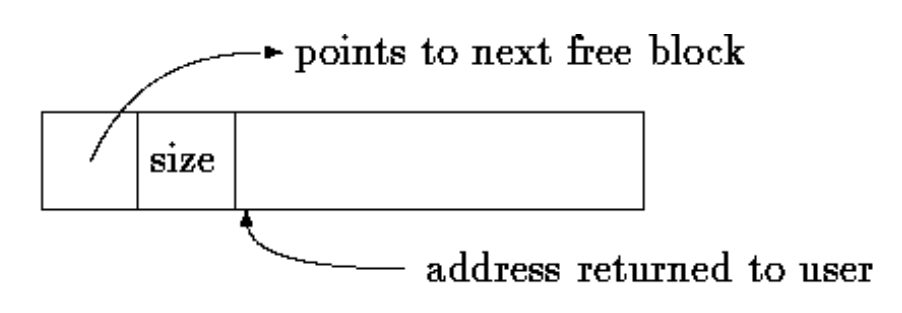
\includegraphics[width=0.4\textwidth]{imagenes/vmm_kmalloc_block.png}}
\caption{Un bloque de memoria del heap}
\end{figure}

\begin{figure}[H]
\centering
\subfloat{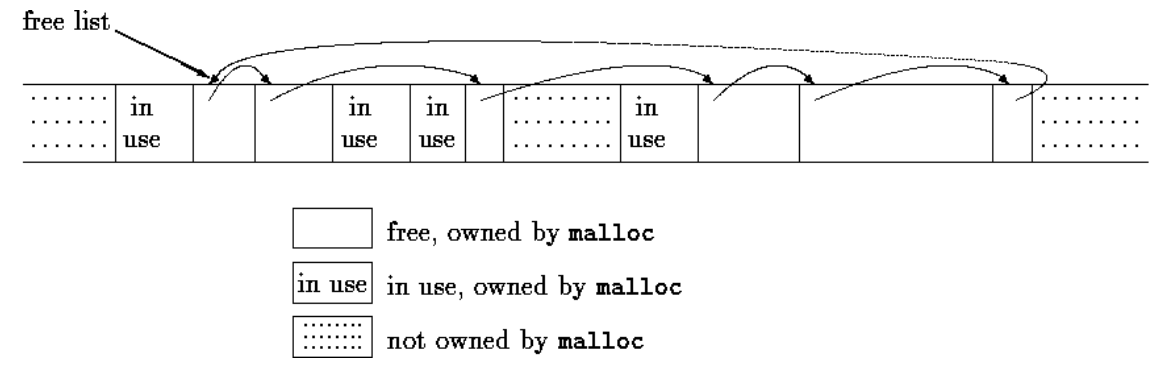
\includegraphics[width=0.4\textwidth]{imagenes/vmm_kmalloc_heap.png}}
\caption{Un bloque de memoria del heap}
\end{figure}

\subsubsection{ kmalloc }
La definicin de kmalloc es la siguiente

\begin{verbatim}
/**
 * Devuelve un puntero a block_size bytes listos para usar dentro del heap del kernel
 * No realiza verificacion de limites, por lo que escribir mas alla del tamao pedido puede ocasionar sobreescribir estructuras de control
 *
 * @param block_size Tamao del nuevo bloque pedido
 * @return ptr_t Puntero al bloque de memoria solicitado
 * @see kfree
 */
ptr_t kmalloc(uint32_t block_size);
\end{verbatim}

El algortmo usado por kmalloc es \textit{First fit}, es decir, cuando kmalloc busca un bloque de tamao block\_size, no busca el mejor para fragmentar menos la memoria, sino que usa el primero que encuentra de tamao mayor o igual. Si el bloque coincide con el tamao solicitado, entonces usa ese. Si en cambio encuentra primero un bloque de tamao mayor, divide el bloque en dos nuevos bloques: uno del tamao solicitado, y otro del tamao restante. Y devuelve el nuevo bloque creado. Si no encuentra bloques para alojar el tamao solicitado, pide al kernel ms espacio para el heap (no intenta reacomodar los bloques libres para generar uno de mayor tamao).

\subsubsection{ kfree }
Kfree esta definida como
\begin{verbatim}
/**
 * Libera un bloque de memoria solicitado con kmalloc.
 *
 * @param prt Puntero al bloque de memoria conseguido con kmalloc
 * @see kmalloc
 */
void kfree(ptr_t ptr);
\end{verbatim}

Kfree al igual que kmalloc libera la memoria siguiendo un algoritmo \textit{First fit}. Recorre el heap buscando una posicin para liberar el bloque. Si encuentra un bloque libre, entonces fusiona ambos bloques para generar uno de mayor tamao y asi reducir la fragmentacin.\\
Cabe aclarar que kfree nunca pide que el heap se achique, siempre se generan bloques ms grandes. Podra eventualmente detectar bloques excesivamente grandes 
y pedir al kernel que libere esas páginas.

\subsubsection{morecore}
La funcin \textit{morecore} es invocada por kmalloc cuando necesita ms espacio para el heap. La definicin es:
\begin{verbatim}
/**
 * Intenta agrandar el heap del kernel reservando mas espacio usand vmm_resize_heap.
 * 
 * @param size Tamao a agrandar
 * @return header_t* Devuelve un puntero al bloque de memoria conseguido, o NULL si no pudo agrandar el heap.
 * @see 
 */
static header_t* vmm_morecore(uint32_t size);
\end{verbatim}
La funcin de morecore es determinar cuntos bytes va a solicitar al kernel, para luego hacer la solicitud mediante la función \textit{vmm\_resize\_heap}

\subsubsection{vmm\_resize\_heap}
\begin{verbatim}
/**
 * Agranda el heap en nbytes bytes.
 *
 * @param nbytes Cantidad de bytes para agrandar el heap
 * @return uint8_t* Puntero al bloque de nbytes bytes.
 * @see vmm_morecore
 */
static uint8_t* vmm_resize_heap(uint32_t nbytes);
\end{verbatim}
Dentro de vmm\_resize\_heap se determina la cantidad entera de pginas de 4kb que son necesarias pedir a la mmu, y el pedido se realiza utilizando la funcin \textit{mmu\_alloc\_at\_VA}. Se especifica la VA del pedido para que el heap se agrande manteniendo la continuidad de las direcciones y asi poder pedirle a kmalloc bloques de ms de 4kb y que funcione correctamente.